%---------------------- begin chap 2 -------------
\cchapter{مفاهیم اولیه}
\label{chap:lit}
\pagebreak

\section {قلب و نحوه‌ی عملکرد آن}
قلب ماهیچه‌ای متشکل از ۴ حفره است. دو حفره‌ی بالایی، دهلیزهای چپ و راست نامیده می‌شوند و دو حفره‌ی پایینی، بطن‌های چپ و راست نام دارند. در هر سیکل تپش قلب، خونِ بدون اکسیژن از طریق بزرگ‌سیاهرگ‌های بالایی و پایینی وارد دهلیز راست می‌شود. پس از طی فرایندی در قلب، خون دارای اکسیژن شده و از بطن چپ خارج می‌شود. این خون سپس از طریق سرخرگ‌ها به اعضای بدن می‌رسد. قلب یک فرد بزرگسال سالم، به طور متوسط بین ۶۰ تا ۱۰۰ بار در دقیقه می‌تپد. \cite{MayoClinic}

عملکرد قلب توسط یک سیستم الکتریکی و به وسیله‌ی سیگنال‌های تولید شده در آن کنترل می‌شود. این سیگنال‌ها دیواره‌های قلب را تحریک می‌کنند و با انقباض دیواره‌ها، خون از قلب خارج شده و در سیستم گردش خون جریان می‌یابد. در ادامه به طور دقیق به نحوه‌ی عملکرد قلب می‌پردازیم. 


\subsection {سیستم هدایت الکتریکی قلب}
تمامی فعالیت‌های قلب که منجر به پمپ‌کردن خون در بدن می‌شوند، تحت کنترل سیستم هدایت الکتریکی قلب \LTRfootnote{Cardiac conduction system} قرار دارند. این سیستم با انتقال الکتریکی سیگنال‌های تولید شده، باعث به تپش درآمدن ماهیچه‌ی قلب می‌شود. بخش‌های اصلی این سیستم عبارت اند از:

\begin{enumerate}
	\item گره سینوسی‌دهلیزی \LTRfootnote{Sinoatrial node} \lr{(SA)} در دهلیز 
	راست قلب
	\item گره دهلیزی‌بطنی \LTRfootnote{Atrioventricular node} \lr{(AV)} در سپتوم داخل‌دهلیزی قلب \LTRfootnote {Interatrial septum} (دیواره‌ای ماهیچه‌ای که دهلیز راست و چپ قلب را جدا می‌کند)
	\item سیستم هیس-پورکینژ \LTRfootnote{His-Purkinje system} در دیواره‌های بطن‌های قلب
\end{enumerate}
این بخش‌ها در شکل \ref{fig:conduction} قابل مشاهده هستند.

\begin{figure}
\centering
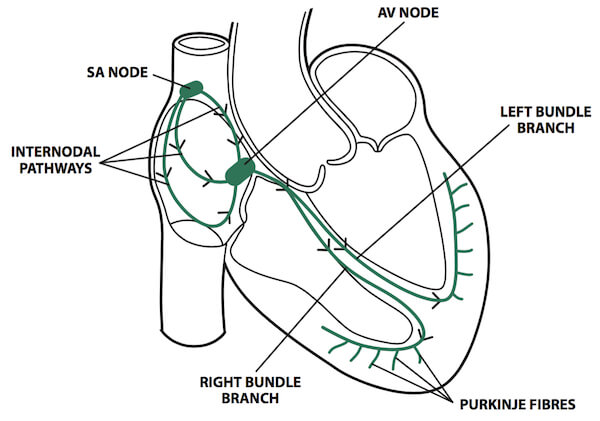
\includegraphics[width=12cm]{Figures/conduction.jpg}
\caption{سیستم هدایت الکتریکی قلب\cite{Medicalexamprep}}
\label{fig:conduction}
\end{figure}

نقطه‌ی آغاز هر ضربان قلب، گره سینوسی‌دهلیزی است. این گره با تولید سیگنالی هر دو دهلیز را تحریک به انقباض می‌کند و در نتیجه‌ی این عمل، خون از طریق دریچه‌های باز، از دو دهلیز وارد دو بطن قلب می‌شود. سپس سیگنال وارد گره دهلیزی‌بطنی شده و برای لحظه‌ای کوتاه تاخیر می‌کند، تا خون فرصت پر کردن دو بطن قلب را پیدا کند. 

در مرحله‌ی بعد، سیگنال آزاد شده و در مسیری به نام دسته‌ی هیس \LTRfootnote{Hiss bundle} واقع در دیواره‌های بطن‌ها حرکت خود را ادامه می‌دهد. در این مرحله، سیگنال به دو دسته تقسیم شده و این دو دسته از طریق دو مسیر به نام‌های فیبرهای پورکینژ \LTRfootnote{Purkinje fibers} چپ و راست، به ترتیب وارد بطن چپ و راست قلب می‌شوند. این عمل باعث انقباض دو بطن می‌شود و در نتیجه‌ی این عمل، خون از طریق دریچه‌های بیرونی قلب، از آن خارج شده و به ریه‌ها و بقیه‌ی اعضای بدن انتقال می‌یابد. در این مرحله سیگنال از بطن‌ها گذر می‌کند و دو بطن وارد حالت استراحت می‌شوند، تا سیگنال بعدی فرابرسد.

تولید پی‌در‌پی این سیگنال‌ها، باعث انقباض و استراحت منظم و هماهنگ قلب شده و ضربان قلب را ایجاد می‌کند. در واقع ضربان قلب هر شخص، توسط تعداد دفعاتی در طول یک دقیقه که گره سینوسی‌دهلیزی سیگنال تولید می‌کند تعیین می‌شود. \cite{Heart} 


\section{آریتمی قلبی}
آریتمی قلبی به دسته‌ای از بیماری‌های قلبی اطلاق می‌شود که در آن‌ها، آهنگ تپش قلب حالتی غیرعادی پیدا می‌کند. به طور کلی دلیل رخ دادن آریتمی، عدم انتقال درست سیگنال‌های الکتریکی قلب بیان می‌شود. تعدادی از انواع آریتمی‌ها می‌توانند شدیدا خطرناک و کشنده باشند. اکثر آریتمی‌ها بی خطر شناخته شده‌اند، اما در صورت عدم تشخیص و رسیدگی به موقع می‌توانند زندگی عادی فرد مبتلا را آشفته ساخته یا حیات او را تهدید کنند. 
\subsection{انواع آریتمی قلبی}
آریتمی‌ها بر اساس نوع اختلالی که در ضربان قلب ایجاد می‌کنند، به چهار دسته‌ی کلی تقسیم می‌شوند.
\begin{enumerate}
	\item ضربان‌های زودرس \LTRfootnote{Premature beats}: در این دسته از آریتمی‌ها، قلب ضربا‌ن‌هایی زودرس تولید می‌کند که آهنگ طبیعی تپش آن را مختل می‌کنند. در صورتی که ضربان زودرس در بطن قلب تولید شده‌باشد، ضربان زودرس بطنی\LTRfootnote{Premature Ventricular Complex (PVC)}، و در صورتی که در دهلیز ایجاد شده باشد، ضربان زودرس دهلیزی \LTRfootnote{Premature Atrial Complex (AVC)} نامیده می‌شود.
	\item تاکی‌کاردی فوق بطنی \LTRfootnote{Supraventricular Tachycardia (SVT)}: در این نوع آریتمی، قلب به صورتی غیرعادی تندتر از معمول  (تقریبا بیش از ۱۰۰ ضربان در دقیقه) می‌تپد. \cite{Amboss} این آریتمی‌ها در بین گره سینوسی‌دهلیزی و گره دهلیزی‌بطنی ایجاد می‌شوند. 
	\item آریتمی‌های بطنی \LTRfootnote {Ventricular arrhythmia}:  آریتمی‌هایی که از پایین گره دهلیزی‌بطنی (در سطح بطن قلب) ریشه می‌گیرند در این دسته قرار دارند.
	\item برادی‌کاردی \LTRfootnote{Bradycardia}: در این نوع آریتمی، قلب بیمار آرام‌تر از حالت عادی می‌تپد و نرخ ضربان قلب معمولا پایین‌تر از ۶۰ تپش در دقیقه است.  \cite{Verywellhealth}

\end{enumerate}

\section{سیگنال نوار قلب}
همان طور که گفته شد، سلول‌های گره سینوسی تحریک الکتریکی منظمی را ایجاد می‌کنند که توسط سیستم هدایت الکتریکی موجود در قلب، به بخش‌های دیگر آن انتشار یافته و باعث تپش متناوب قلب می‌شود. نتیجه‌ی این فعالیت، ایجاد جریان الکتریکی در سطح بدن و تحریک تغییرات در پتانسیل الکتریکی سطح پوست است. این سیگنال‌ها را می‌توان به وسیله‌ی الکترودها و دیگر تجهیزات، ثبت و اندازه‌گیری نمود.

در فرایند ثبت نوار قلب، اختلاف پتانسیل بین نقاط قرارگیری الکترودها بر روی بدن اندازه‌گیری شده و معمولا به کمک تقویت‌کننده‌های عملیاتی \LTRfootnote{Operational amplifiers} بهبود داده می‌شود. در مرحله‌ی بعد، سیگنال ابتدا از یک فیلتر بالاگذر و سپس از یک فیلتر پایین‌گذر تصحیح فرکانس عبور داده‌می‌شود. در نهایت این سیگنال آنالوگ، به سیگنال دیجیتال تبدیل می‌شود. منحنی گرافیکی رسم شده در انتهای این فرایند، نوار قلب، و یا به اختصار \lr{ECG} نامیده می‌شود. 

امروزه در روش‌های استاندارد اندازه‌گیری نوار قلب،تعدادی الکترود بر روی سطح پوست قرارمی‌گیرند و یکی از آن‌ها به عنوان مرجع \LTRfootnote{Reference} برای دیگر الکترودها در نظر گرفته می‌شود. به طور معمول، الکترود مرجع روی ساق پای راست نصب می‌شود. \cite{ECGSurvey} هر یک از الکترودهای دیگر، ولتاژ ناحیه‌ی قرارگیری خود را نسبت به ولتاژ الکترود مرجع اندازه‌گیری می‌کنند. هر یک از این اختلاف پتانسیل‌های اندازه‌گیری شده، یک لید \LTRfootnote{Lead} نامیده می‌شود. 
\subsection{نحوه‌ی قرارگیری الکترودها بر روی پوست و لیدهای تولیدشده}

یکی از ترکیب‌های رایج قراردادن الکترودها متشکل از ۱۰ الکترود است که بر روی دست، پا و سینه‌ی بیمار قرار می‌گیرند. از ترکیب این الکترودها ۱۲ لید ایجاد می‌شود که به سه دسته‌ی کلی تقسیم می‌شوند:
\begin{itemize}
	\item  سه لید دوقطبی اندامی \LTRfootnote{Bipolar limb leads} به نام‌های \lr{I}، \lr{II} و \lr{III}
	\item سه لید تک‌قطبی اندامی \LTRfootnote{Unipolar limb leads} به نام‌های \lr{aVF}، \lr{aVL} و \lr{aVR}
	\item شش لید تک‌قطبی سینه‌ای به نام‌های \lr{V1} تا \lr{V6}
\end{itemize}
  هر یک از این لیدها فعالیت الکتریکی قلب را از یک زاویه‌ی خاص در بدن نشان می‌دهد. پرکاربردترین لید برای تشخیص بیماری‌های قلبی، لید \lr{II} می‌باشد که اختلاف پتانسیل بین الکترودهای ساق پای چپ و بازوی راست را نشان می‌دهد. در شکل \ref{fig:leads} یک نوار قلب ۱۲ لیدی مشاهده می‌شود. منحنی رسم شده از هر لید به صورت جداگانه نشان داده شده‌است و لید \lr{II} نیز به تنهایی رسم شده‌است. این لید به خصوص از آن جهت اهمیت دارد که نمای خوبی از ترکیب \lr{QRS}
ارائه می‌دهد. در بخش بعد در مورد این موضوع به تفصیل توضیح داده خواهد شد.
\begin{figure}
\centering
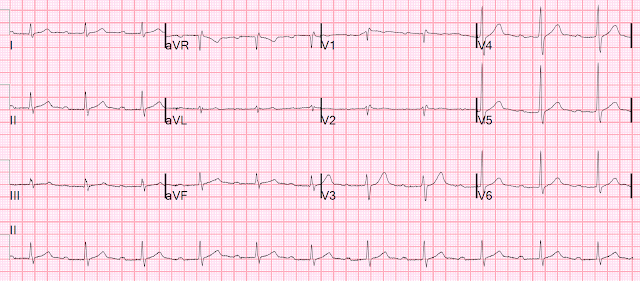
\includegraphics[width=16cm]{Figures/leads.png}
\caption{نوار قلب ۱۲ لیدی گرفته‌شده از یک فرد سالم\cite{Drsmith}}
\label{fig:leads}
\end{figure}

\subsection{ترکیب QRS}
با بررسی یک سیکل ضربان قلب در نوار قلب، ۵ انحراف\LTRfootnote{Deflection}
یا موج پراهمیت دیده می‌شود. اولین موج، \lr{P} نام دارد که با فعال شدن دهلیزهای راست و چپ و بالارفتن پتانسیل الکتریکی آن‌ها اتفاق می‌افتد. سه موج بعدی به ترتیب \lr{Q}، \lr{R} و \lr{S} نام دارند. این سه موج به ترتیب و با فاصله‌ی کمی از هم رخ می‌دهند و عموما به عنوان یک ترکیب، همراه یکدیگر بررسی می‌شوند. این ترکیب که \lr{QRS} نامیده می‌شود، واضح‌ترین بخش مشاهده‌شده در یک سیکل قلبی است که مدت زمان بالارفتن پتانسیل ماهیچه‌های بطنی قلب را نشان می‌دهد. موج بعدی \lr{T} نام دارد که در طول آن بطن‌ها منقبض شده و بار مثبت خود را تخلیه می‌کنند. ترکیب \lr{QRS} در شکل \ref{fig:QRS} مشاهده می‌شود.

\begin{figure}
\centering
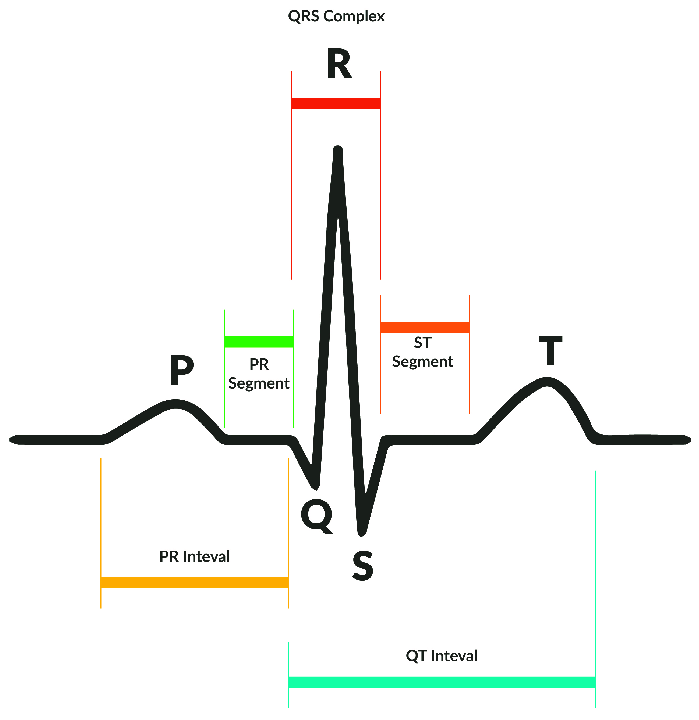
\includegraphics[width=10cm]{Figures/qrs.png}
\caption{ ترکیب \lr{QRS} \cite{Miramontes2017}}
\label{fig:QRS}
\end{figure}
 
\subsubsection{بازه‌های زمانی مهم در سیکل ضربان قلب}
مهم‌ترین بازه‌های زمانی در یک سیکل ضربان قلب عبارت اند از:
\begin{itemize}
	\item بازه‌ی \lr{PR}: فاصله‌ی زمانی از ابتدای موج \lr{P} تا ابتدای ترکیب QRS 
	\item مدت‌زمان \lr{QRS}: مدت‌زمان رخ‌دادن ترکیب \lr{QRS}
	\item بازه‌ی \lr{QT}: فاصله‌ی زمانی از ابتدای ترکیب \lr{QRS} تا انتهای موج \lr{T}
	\item بازه‌ی \lr{RR}: مدت‌زمان سیکل کامل قلب که نشان‌دهنده‌ی سیکل کامل بطن‌ها می‌باشد. 
	\item بازه‌ی \lr{PP}: مدت‌زمان سیکل کامل دهلیزی
\end{itemize}


 \subsubsection{تاثیر آریتمی قلبی بر روی شکل ترکیب QRS}
 وجود آریتمی قلبی می‌تواند باعث تغییر شدید در امواج \lr{Q}، \lr{R} و \lr{S} شود. لید \lr{II} به دلیل واضح‌تر نشان دادن ترکیب \lr{QRS} و لیدهای \lr{V1} تا \lr{V6} به دلیل این که الکترودهای آن‌ها بر روی سینه قرارگرفته و تشخیص بهتر تغییرات پتانسیل ماهیچه‌ی بطنی را ممکن می‌سازند، تا کنون بهترین نتایج را در تشخیص آریتمی نشان داده‌اند. \cite{ECGSurvey}

در طول بازه‌ی زمانی \lr{QRS} بطن‌هابه وسیله‌ی سیستم هیس-پورکینژ منقبض می‌شوند. این سیستم شامل سلول‌هایی در دیواره‌های بطن‌ها است که خاصیت رسانایی سریع الکتریکی را دارند. در صورت ایجاد اختلال در کار این سیستم و ضعیف‌شدن خاصیت رسانایی الکتریکی سلول‌ها، بازه‌ی زمانی \lr{QRS} طولانی‌تر می‌شود. در برخی موارد سیگنال الکتریکی به جای انتقال یافتن از طریق سیستم هیس-پورکینژ، از طریق ماهیچه‌های قلب منتقل می‌شود. این اتفاق منجر به طولانی شدن زمان انتقال الکتریکی سیگنال و در نتیجه عریض شدن بازه‌ی \lr{QRS} می‌شود.
 به طور معمول طول یک بازه‌ی \lr{QRS} بین ۰/۰۸ تا ۰/۱ ثانیه است. در مواردی که طول این بازه از ۰/۱۲ ثانیه بیشتر شود، \lr{QRS} غیرعادی تلقی می‌شود. \cite{Healio}

\section{مسائل دسته‌بندی}

در مسائل دسته‌بندی، ورودی‌های مسئله تعدادی داده هستند و مطلوب مسئله، جای دادن هر یک از داده‌ها در یک دسته یا کلاس است. به بیان رسمی‌تر در این مسئله‌ها، هدف، تخمین‌زدن یک نگاشت از متغیرهای ورودی \lr{X} به تعدادی متغیر خروجی گسسته \lr{Y} است. این متغیرهای خروجی تعدادی برچسب\LTRfootnote{Label} هستند که تعیین می‌کنند هر داده در کدام دسته قرار می‌گیرد. تعداد این دسته‌ها می‌تواند دو و یا بیشتر باشد که در حالت دوم، مسئله یک مسئله‌ی دسته‌بندی چنددسته‌ای\LTRfootnote{Multiclass classification problem} نامیده می‌شود. 

\subsection{روش ماشین بردار پشتیبانی (SVM)}
یکی از پرکاربردترین دسته‌های الگوریتم برای حل مسایل دسته‌بندی، الگوریتم‌های \lr{SVM} هستند. در این الگوریتم‌ها، داده‌ها به مثابه‌ی نقطه‌هایی در یک فضای \lr{N}بعدی فرض می‌شوند. هدف الگوریتم، یافتن ابرصفحه‌هایی\LTRfootnote{Hyperplanes} است که به طور بهینه نقطه‌های داده‌ها را به کلاس‌های متعدد دسته‌بندی کند. تعداد بعدهای این فضا \lr{(N)} برابر با تعداد ویژگی‌ها است. معمولا تعداد زیادی ابرصفحه را می‌توان برای جداسازی دو کلاس مختلف از داده‌ها یافت، اما در این الگوریتم، هدف یافتن ابرصفحه‌ای است که بیشترین فاصله را با نزدیک‌ترین نقطه‌ی داده در هر یک از کلاس‌ها داشته‌باشد. این فاصله، حاشیه\LTRfootnote{Margin} نامیده می‌شود. 

\subsubsection{ابرصفحه}
ابرصفحه مرزی است که نقاط داده‌ها را در یک فضای \lr{N}بعدی به دو بخش تقسیم می‌کند. برای مثال در مسئله‌ای با دو کلاس هدف، نقاطی که در هر یک از دو سمت ابرصفحه‌ی به‌دست‌آمده قرار می‌گیرند، به یکی از آن دو کلاس تعلق می‌یابند. تعداد بعد ابرصفحه بسته به تعداد ویژگی‌های داده‌ها است. مثلا در مسئله‌ای که سه ویژگی برای داده‌ها به دست آورده‌ایم، فضای داده ۳بعدی بوده و در نتیجه ابرصفحه‌ی جداکننده‌ی داده‌ها نیز ۳بعدی خواهد بود.

\subsubsection{بردار پشتیبانی}
بردارهای پشتیبانی، نقاط داده‌ای هستند که ابرصفحه را تعریف می‌کنند. این نقاط به ابرصفحه نزدیک‌تر بوده و بر روی موقعیت قرارگیری و جهت آن تاثیر می‌گذارند. به کمک این بردارها، ابرصفحه‌ای با بیشترین حاشیه برای دسته‌بندی انتخاب می‌شود.\cite{SVM} نمودار یک مسئله‌ی دسته‌بندی دوبعدی در شکل \ref{fig:SVMClassification} دیده می‌شود.

\begin{figure}
\centering
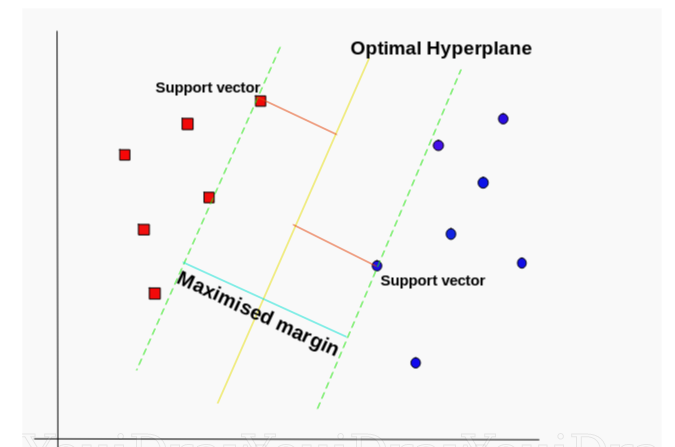
\includegraphics[width=10cm]{Figures/svmMargin.png}
\caption{ نموداری از حل یک مسئله‌ی دسته‌بندی دوبعدی با روش \lr{SVM}\cite{SVM}}
\label{fig:SVMClassification}
\end{figure}
 

\subsubsection{ تابع کرنل}
در روش \lr{SVM} برای دسته‌بندی داده‌ها از توابعی به نام توابع کرنل استفاده می‌شود. تابع کرنل داده را به عنوان ورودی گرفته و آن را به فضایی دیگر انتقال \LTRfootnote{Transform} می‌دهد. به کمک تابع کرنل، داده‌هایی که در فضای عادی مشاهده شده‌اند، به فضایی با تعداد ابعاد بالاتر انتقال می‌یابند که در چنین فضایی امکان جداسازی آن‌ها وجود دارد. در واقع هر مدل خطی را می‌توان به کمک تابع کرنل به یک مدل غیر خطی تبدیل کرد، به این صورت که ویژگی‌های مدل را با یک تابع کرنل جایگزین کنیم. 

به طور رسمی‌تر می‌توان تابع کرنل را به این صورت تعریف کرد: به ازای هر  $x$  و $x'$ در فضای $X$ می‌توان توابعی به صورت $k(x, x')$ را یافت که حاصل ضرب داخلی دو نقطه در فضای دیگری به نام $V$ است. این روابط در معادله‌ی \ref{eq:kernel} قابل مشاهده است.\cite{KernelSVM} 

\begin{equation}
\begin{split}
	& k: X \times X \to \mathbb{R} \\
	& k(x_i, x_j) = \bigg \langle \Phi (X_i), \Phi(X_j) \bigg \rangle
\end{split}
\label{eq:kernel}
\end{equation}

ساده‌ترین نوع کرنل، کرنل خطی است. این توابع  داده‌ها را به فضایی با تعداد بعد بالاتر نگاشت نمی‌کنند، به همین دلیل بهتر است در مسائلی که داده‌ها به صورت خطی قابل جداسازی هستند، از این نوع کرنل استفاده شود. 
 این نوع کرنل‌ها به دلیل سادگی و خطی بودن، سرعت بیشتری در دسته‌بندی دارند. معمولا در مسائلی که تعداد ویژگی‌ها زیاد بوده و نگاشت داده‌ها به نقاطی در فضای با تعداد بعدهای بالاتر تاثیر چشمگیری در بهبود دسته‌بندی ندارد، از کرنل خطی استفاده می‌شود. \cite{LinearSVM} 
 نوع پیچیده‌تری از کرنل که در بسیاری از مسائل دسته‌بندی کاربرد دارد. کرنل \lr{RBF}\LTRfootnote{ Radial Basis Function} نام دارد. این تابع بر روی نقطه‌ی $X_i$ و $X_j$ در فضای $X$ که یک فضای ورودی است در معادله‌ی \ref{eq:kernelRBF} قابل مشاهده است.\cite{kernelRBF}
   
\begin{equation}
	 k(X_i, X_j) = \exp(-\frac{{||X_i-X_j||}^2}{2\sigma^2})
\label{eq:kernelRBF}
\end{equation}
در این رابطه $\sigma$ یک پارامتر آزاد است. این تابع، دو بردار $X_i$  و $X_j$ که در فضایی دو بعدی قرار دارند را به یک بردار بی‌نهایت نگاشت می‌کند. این عمل باعث می‌شود نقاط داده به نقاطی در فضایی با تعداد بعد بیشتر نگاشت شوند. در مسائلی که در فضای اصلی داده‌های ورودی، ابرصفحه‌ای برای جداسازی کلاس‌ها یافت نمی‌شود، می‌توان با استفاده از کرنل \lr{RBF} در فضایی با تعداد بعد بالاتر، ابرصفحه‌ای برای جداسازی کلاس‌ها یافت. این موضوع در شکل \ref{fig:RBFKernel} قابل مشاهده است. این نوع تابع کرنل، زمان و قدرت پردازشی بیشتری به نسبت کرنل خطی مصرف می‌کند.

\begin{figure}
\centering
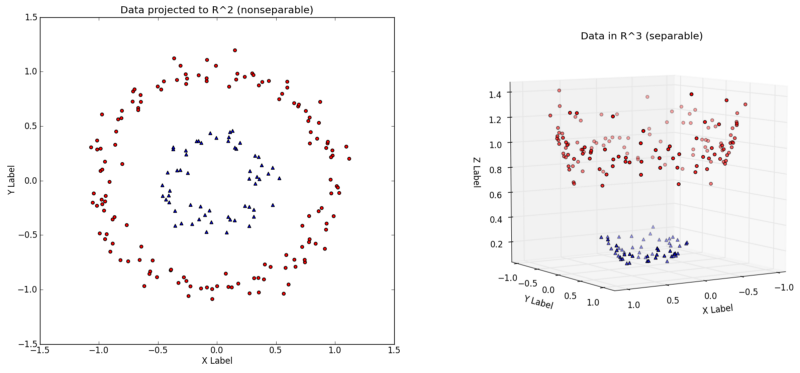
\includegraphics[width=15cm]{Figures/RBFKernel.png}
\caption{ سمت چپ: داده‌های غیر قابل جداسازی توسط یک ابرصفحه در یک فضای دوبعدی، سمت راست: داده‌های انتقال‌داده‌شده به فضای سه‌بعدی و قابل جداسازی\cite{TowardsScienceRBF}}
\label{fig:SVMClassification}
\end{figure}

\subsubsection{ انجام دسته‌بندی  با استفاده از تابع کرنل RBF}
برای انجام عمل دسته‌بندی با استفاده از کرنل \lr{RBF}، لازم است تعدادی پارامتر برای این تابع تعیین شوند. میزان تاثیر هر یک از این پارامترها بر روی نتیجه‌ی نهایی دسته‌بندی معمولا به کاربرد وابسته است. در ادامه تعدادی از  مهم‌ترین پارامترها توضیح داده می شوند. 
\begin{itemize}
	\item پارامتر $\gamma$:
	\\
	$\gamma$ پارامتر آزادی است که در تابع کرنل \lr{RBF} وجود دارد. این پارامتر تعیین می‌کند یک داده به تنهایی چقدر می‌تواند بر روی نتیجه‌ی نهایی دسته‌بندی تاثیر داشته‌باشد. در صورت کوچک‌بودن $\gamma$ این تاثیر زیاد و در صورت بزرگ‌بودن آن، این تاثیر کم است. این پارامتر را می‌توان به صورت عکس شعاع تاثیر نمونه‌هایی که مدل به عنوان بردار ساپورت انتخاب می‌کند دانست. گامای کوچک باعث می‌شود منحنی گاوسی تابع کرنل، واریانس زیادی داشته‌باشد. اگر $X_j$ یک بردار ساپورت باشد، کوچک‌بودن $\gamma$ نتیجه می‌دهد که کلاس این بردار ساپورت، بر روی تشخیص کلاس $X_i$  تاثیر دارد حتی اگر فاصله‌ی آن‌ها زیاد باشد. برعکس اگر $\gamma$ بزرگ باشد، واریانس کوچک بوده و این نتیجه می‌دهد یک بردار ساپورت تاثیر زیادی بر روی تشخیص کلاس نمونه‌ها ندارد.

رفتار مدل نسبت به مقدار $\gamma$ بسیار حساس است. به طور کلی می‌توان گفت بزرگ‌بودن بیش از حد $\gamma$ باعث می‌شود شعاع ناحیه‌ای که بردار ساپورت بر روی آن تاثیر دارد بسیار کوچک شده و تنها خود بردار را در بر بگیرد. کوچک‌بودن بیش از حد آن نیز باعث می‌شود ناحیه‌ی تاثیر هر یک از بردارهای ساپورت به اندازه‌ی کل مجموعه‌ی داده‌ها بزرگ می‌شود و مدل نهایی تفاوتی با یک کرنل خطی که در آن تعدادی ابرصفحه نقاط داده را از هم جدا می‌کنند نخواهد داشت.

	\item پارامتر $C$:
	\\
	در \lr{SVM} هدف پیدا کردن مرز جداکننده‌ای است که تمامی داده‌های مربوط به هر یک از کلاس‌ها را به درستی جدا کند. در صورت وجود خطا در نمونه‌ها و یا داده‌های غیرعادی، این کار باعث می‌شود مدل نتواند مرز مناسبی برای جداسازی کلاس‌ها بیابد. به همین علت مفهوم حاشیه‌ی نرم\LTRfootnote{Soft margin} مطرح می‌شود. با اعمال حاشیه‌ی نرم، به \lr{SVM} اجازه داده می‌شود برخی از نمونه‌ها را در دسته‌بندی در نظر نگیرد و برخی از نمونه‌ها را در کلاس نادرست دسته‌بندی کند. پارامتر $C$ شدت این عمل را کنترل می‌کند. این پارامتر تاثیر هر یک از بردارهای ساپورت بر روی حاشیه‌ی ابرصفحه‌ی جدا کننده را نشان می‌دهد. مدلی با $C$ پایین‌تر، آسان‌گیرانه تر دسته‌بندی کرده و منجر به داشتن داده‌های بیشتری با دسته‌بندی نادرست می‌شود، اما در عوض حاشیه‌ی بالاتری را نتیجه می‌دهد. 
\end{itemize} 
 

\subsection{دسته‌بندی داده‌ها با استفاده از روش SVM}
روش کلی ساخت یک مدل \lr{SVM} به این صورت است که داده‌ها را به دو مجموعه‌ی داده‌های آموزشی\LTRfootnote{Training data set} و داده‌های تست\LTRfootnote{Test data set} تقسیم می‌کنیم. نحوه‌ی تقسیم داده‌ها به این دو مجموعه تا حد زیادی به مسئله وابسته است. نحوه‌ی کلی انجام دسته‌بندی به این صورت است که ابتدا عملیات آموزش بر روی مجموعه‌ی اول انجام شده و مدل SVM ساخته می‌شود. سپس این مدل بر روی محموعه‌ی تست آزموده شده و دقت دسته‌بندی، با توجه به معیارهای کارایی مورد نظر در مسئله اندازه‌گیری می‌شود.

 \subsubsection{تعیین پارامترهای مدل با استفاده از روش اعتبارسنجی متقابل }
 در هنگام ساخت مدل \lr{SVM} پارامترهایی مانند پارامتر \lr{C} باید به صورت دستی برای مدل تعیین شوند. ممکن است مقداری که برای یک پارامتر در مدل تعیین می‌شود، به نحوی دست‌کاری شود که مدل به‌دست‌آمده دقت خوبی در دسته‌بندی داده‌های تست داشته‌باشد، اما بر روی داده‌های ناشناخته‌ی دیگر این دقت را تضمین نکند. در چنین حالتی پارامترها تنها به هدف بالابردن دقت دسته‌بندی در داده‌های مجموعه‌ی تست تعیین شده‌اند و در واقع مدل، دانشی از مجموعه‌ی تست دارد. ارزیابی مدل در این شرایط نمی‌تواند مفید باشد، چرا که میزان موفقیت آن در دسته‌بندی داده‌های جدیدی که هیچ پیش‌فرضی از آن‌ها ندارد، پایین‌تر از مقدار به‌دست‌آمده خواهد بود.

در این شرایط، از روشی به نام اعتبارسنجی متقابل\LTRfootnote{Cross-validation} برای تعیین پارامترهای الگوریتم، به خصوص \lr{C} استفاده می‌شود. در اعتبارسنجی متقابل \lr{k} لایه‌ای\LTRfootnote{K-fold cross-validation}، مجموعه‌ی آموزش به \lr{k} بخش تقسیم می‌شود، سپس مدلی با استفاده از داده‌های \lr{k} بخش از این بخش‌ها آموزش داده شده و بر روی یک بخش باقی‌مانده آزموده می‌شود. این عمل \lr{k} بار برای هر \lr{k} بخش موجود اجرا خواهد شد. در انتها معیارهای کارایی گزارش‌شده توسط این روش، میانگین معیارهای کارایی به‌دست‌آمده  در هر یک از لایه‌ها خواهد بود. این عمل برای مقادیر مختلفی از پارامتر مورد نظر، مثلا \lr{C}، اجرا شده و مقداری که بهترین معیارهای کارایی را نتیجه دهد، به عنوان مقدار پارامتر تعیین می‌شود.


\section{معیارهای کارایی در مسائل دسته‌بندی}

پس از استخراج ویژگی‌ها و آموزش مدل دسته‌بندی، باید میزان موفقیت الگوریتم در دسته‌بندی داده‌های تست سنجیده شود. برای این منظور، معیارهای استانداردی تعریف شده‌اند. پیش از پرداختن به این معیارها لازم است با مقادیر مثبت و منفی صحیح و کاذب در مسائل دسته‌بندی چنددسته‌ای آشنا شویم.

در یک مسئله‌ی دسته‌بندی چند دسته‌ای مقادیر زیر برای هر کلاس تعریف می‌شوند:
\begin{itemize}
	\item مثبت صحیح\LTRfootnote{True Positve} \lr{(TP)}: داده‌هایی که به درستی در این کلاس دسته‌بندی شده‌اند.
	\item مثبت کاذب\LTRfootnote{False Positive} \lr{(FP)}: داده‌هایی که در دسته‌بندی متعلق به این کلاس تشخیص داده شده‌اند اما در واقعیت به کلاس دیگری تعلق دارند.
	\item منفی صحیح\LTRfootnote{True Negative} \lr{(TN)}: داده‌هایی که عدم تعلق آن‌ها به این کلاس به درستی تشخیص داده شده است.
	\item منفی کاذب\LTRfootnote{False Negative} \lr{(FN)}: داده‌هایی که الگوریتم آن‌ها را متعلق به کلاس‌های دیگر تشخیص داده‌است، اما در واقع به این کلاس تعلق دارند.
\end{itemize}

\subsection{ماتریس درهم‌ریختگی}
ماتریس درهم‌ریختگی\LTRfootnote{Confusion matrix} یک ماتریس مربعی است که برای مشاهده و ارزیابی نتایج الگوریتم‌های دسته‌بندی به کار می‌رود. تعداد سطرها و ستون‌های این ماتریس به تعداد کلاس‌های هدف است. یکی از محورهای ماتریس، برچسب‌های پیش‌بینی‌شده توسط مدل برای داده‌های مجموعه‌ی تست و محور دیگر، برچسب‌های واقعی آن داده‌ها را نشان می‌دهد. در شکل \ref{fig:confusionmatrix} ماتریس درهم‌ریختگی یک مسئله‌ی دسته‌بندی چنددسته‌ای را مشاهده می‌کنیم. درایه‌ی $[x, y]$ در این ماتریس نشان می‌دهد چه تعداد داده وجود دارد که به وسیله‌ی الگوریتم آن‌ها در دسته‌ی $x$ جای داده شده‌اند، اما در واقع به دسته‌ی $y$ تعلق دارند. درایه‌های قطری نشان‌دهنده‌ی مثبت‌های صحیح برای هر کلاس هستند. از این ماتریس می‌توان مقادیر مفیدی برای ارزیابی مدل‌های دسته‌بندی استخراج نمود.

\begin{figure}[!htb]
\centering
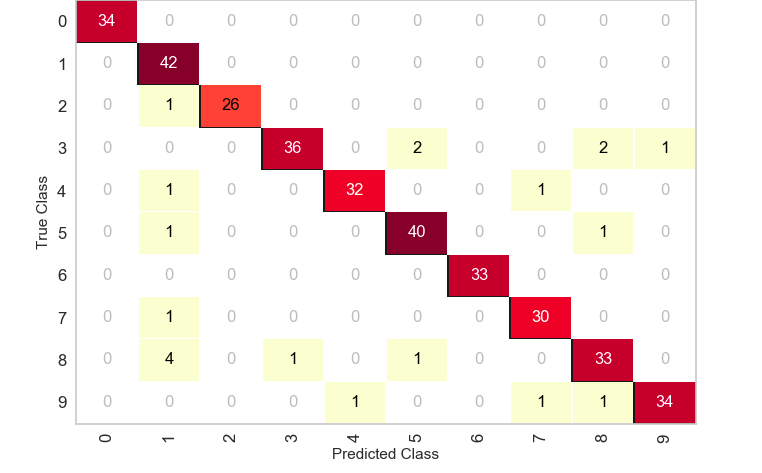
\includegraphics[width=14cm]{Figures/confusionmatrix.png}
\caption{ ماتریس درهم‌ریختگی برای یک مسئله‌ی دسته‌بندی چنددسته‌ای \cite{Confusion}}
\label{fig:confusionmatrix}
\end{figure} 

\subsection{دقت و حساسیت}
در یک مسئله‌ی دسته‌بندی چند دسته‌ای، برای هر دسته مقادیر دقت\LTRfootnote{Precision} و حساسیت\LTRfootnote{Sensitivity} تعریف می‌شوند. دقت دسته‌بندی برای کلاس \lr{A} (که نرخ پیش‌بینی‌پذیری مثبت\LTRfootnote{Positive predictivity} نیز نامیده می‌شود) نشان می‌دهد چقدر احتمال دارد که داده‌ای که در \lr{A} دسته‌بندی شده است، واقعا به این دسته تعلق داشته باشد. رابطه‌ی \ref{eq:precision} نحوه‌ی محاسبه‌ی دقت را نشان می‌دهد.
\begin{equation}
	 Precision = \frac{TP}{TP+FP}
\label{eq:precision}
\end{equation}
حساسیت محاسبه‌شده برای کلاس \lr{A} نشان می‌دهد چقدر احتمال دارد داده‌ای که در واقع به کلاس  \lr{A} تعلق دارد، در این کلاس دسته‌بندی شود. رابطه‌ی \ref{eq:sensitivity} نحوه‌ی محاسبه‌ی این مقدار را نشان می‌دهد.
\begin{equation}
	 Sensitivity = \frac{TP}{TP+FN}
\label{eq:sensitivity}
\end{equation}

\subsection{صحت و صحت کلی}
صحت\LTRfootnote{Accuracy} به صورت رابطه‌ی \ref{eq:accuracy} تعریف می‌شود. این مقدار را می‌توان برای هر کلاس به صورت جدا محاسبه کرد، که در این صورت نسبت داده‌هایی که به درستی متعلق به یک کلاس تشخیص داده شده اند به کل داده‌هایی که در آن کلاس دسته‌بندی شده‌اند را نشان می‌دهد. صحت را می‌توان برای تمامی کلاس‌ها نیز محاسبه کرد، که در این صورت  به آن صحت کلی\LTRfootnote{Overall accuracy} گفته می‌شود. صحت کلی، نسبت داده‌هایی که به درستی در تمام دسته‌ها دسته‌بندی شده‌اند به کل داده‌های تست را نشان می‌دهد.
\begin{equation}
	 Accuracy = \frac{TP+TN}{TP+FP+TN+FN}
\label{eq:accuracy}
\end{equation}